\chapter{树与二叉树}\label{DS05}

\par\medskip\noindent\textbf{章节脉络}\par\smallskip
\begin{wideblock}\centering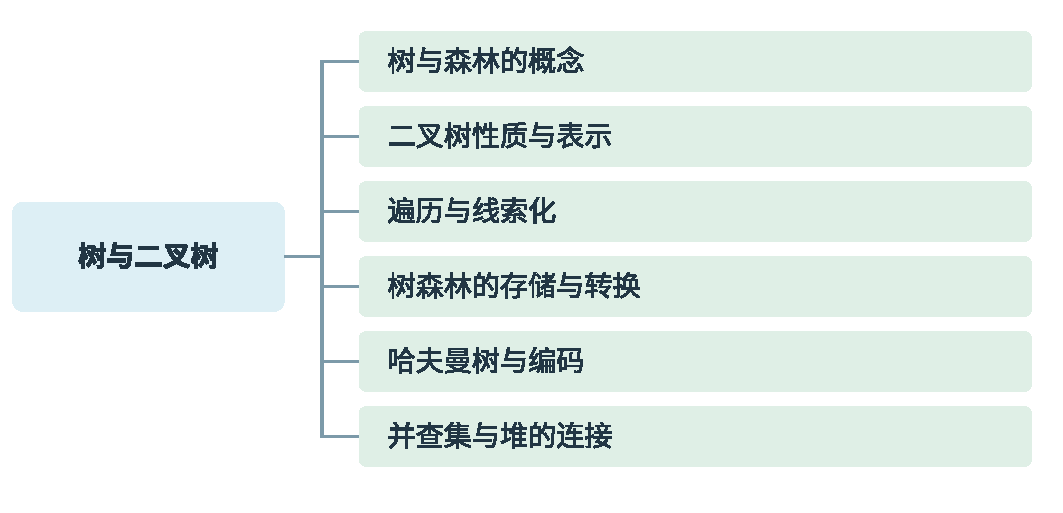
\includegraphics[width=\linewidth,height=92mm,keepaspectratio]{figures/overview.pdf}\end{wideblock}\par\medskip

树用父子关系组织层次。二叉树在此基础上区分左、右位置，遍历把结构转成一个处理次序；哈夫曼树、并查集和堆则各自增加约束，分别处理编码、集合合并和最值访问。它们共享树的表示工具，但各自的性质不能互相替代。

\section{本章知识结构}\label{DS05-map}

\begin{itemize}
\tightlist
\item
  \textbf{树与森林的概念}：结点与父子兄弟；有序树与无序树；结点度与树度；层次高度与路径；边数及叶数计数。
\item
  \textbf{二叉树性质与表示}：满与完全二叉树；叶数与双孩子结点；顺序编号及空位；二叉链表空域。
\item
  \textbf{遍历与线索化}：先中后序及层序；非递归栈状态；遍历序列还原；中序线索与标志；前驱后继及边界。
\item
  \textbf{树森林的存储与转换}：双亲表示；孩子表示；孩子兄弟表示；左孩子右兄弟转换；先根后根与二叉遍历。
\item
  \textbf{哈夫曼树与编码}：带权路径长度；合并两个最小权根；最优性与编码非唯一；前缀编码与剩余容量；多路归并的零权补叶。
\item
  \textbf{并查集与堆的连接}：双亲森林与代表元；按规模合并；路径压缩不改集合；完全性与堆序；插入上滤及删根下滤。
\end{itemize}

树的概念和计数性质是后续推导的基础。读遍历时同时追踪程序、栈或队列与输出序列；读编码和并查集时，再考察它们各自增加的约束。

\section{树的结点、度、层次与路径}\label{DS05-01}

\begin{definition}[树及结点的度]

\textbf{有序树}规定同一结点各子树的先后，交换两个孩子可能改变树；\textbf{无序树}不区分这种先后。森林是零棵或多棵互不相交的树，删去一棵非空树的根后，各子树构成森林；在一片森林上加新根、把各棵树根接为孩子，又得到一棵树。普通树的有序性与``关键字从小到大''无关。

非空树有且仅有一个根。除根外每个结点恰有一个双亲，根到任意结点只有一条简单路径；树的各子树互不相交。一个结点的孩子数称为该结点的\textbf{度}，树的度是所有结点度的最大值。度为0的结点称为叶结点。树中``度''通常指数孩子的个数，与无向图把关联边条数称为度的约定不同。

\end{definition}

本章按王道课件约定，根为第1层，结点的层次（深度）从根向下按层计，树的高度（深度）为最大层号；结点高度从该结点向下到最深叶子按层计，叶子高度为1，空树高度为0。根到结点的路径长度仍按边数计，等于该结点层次减1。题目若另行按边数定义高度或深度，须先换算全部相关公式。

路径长度以边数计，不以沿途结点数计。树的路径长度是根到各结点路径长度的总和；树高由最长的一条路径决定，二者不同。孩子、子孙、兄弟也要区分：兄弟共有同一个双亲，与堂兄弟不是同一个概念。

\subsection{例 5-1　怎样从非叶结点数求叶结点数}\label{DS05-ex1}

\begin{example}[配套案例]

【配套例题】 一棵度为4的树，含20个度为4的结点、10个度为3的结点、1个度为2的结点、10个度为1的结点。叶结点数为（　）。

A. 41　B. 82　C. 113　D. 122

\end{example}

\textbf{解析。} 设叶数为 \(n_0\)。一方面总结点数为 \(n=n_0+20+10+1+10=n_0+41\)；另一方面每条边从一个双亲指向一个孩子，边数是度数总和 \(4\times20+3\times10+2+10=122\)。树有 \(n-1\) 条边，所以 \(n_0+40=122\)，得 \(n_0=82\)，答案为 \textbf{B}。

一般地，令 \(n_i\) 为度为 \(i\) 的结点数，由 \(\sum_i n_i-1=\sum_i i n_i\) 得

\[n_0=1+\sum_{i\ge2}(i-1)n_i.\]

度为1的结点不出现在右端，是因为在一条边上再串入一个单孩子结点，结点数、边数各增加1，叶数不变。因此只给定 \(n_2,n_3\) 和叶数，未必能确定全树结点总数；还可能插入任意多个度为1的结点。

每结点至多有 \(m\) 个孩子的树，第 \(i\) 层至多有 \(m^{i-1}\) 个结点，高度 \(h\) 至多容纳 \((m^h-1)/(m-1)\) 个结点（\(m>1\)）。求最小高度时，找使容量至少达到 \(n\) 的最小整数 \(h\)。例如至多3叉、50个结点，高4时最多40个，高5时最多121个，所以最小高度5。这里必须把``度为3''理解为全树最大孩子数3，不能要求每个非叶结点都恰有3个孩子。

\subsection{\texorpdfstring{度为\(m\)的树与\(m\)叉树}{度为m的树与m叉树}}\label{DS05-mary}

``度为\(m\)''要求全树至少有一个结点恰有\(m\)个孩子；``\(m\)叉树''只要求每个结点至多有\(m\)个孩子。二者都满足每层的容量上界，最少结点数却不同。对非空树，按根为第1层：

\par\medskip\noindent\begin{minipage}{\linewidth}\fontsize{9.3}{12}\selectfont\begin{tabularx}{\linewidth}{@{}YYY@{}}
\toprule\noalign{}
\begin{minipage}[b]{\linewidth}\raggedright
条件
\end{minipage} & \begin{minipage}[b]{\linewidth}\raggedright
最少结点数
\end{minipage} & \begin{minipage}[b]{\linewidth}\raggedright
最多结点数
\end{minipage} \\
\midrule\noalign{}


高度\(h\)的\(m\)叉树 & \(h\)，取一条单支链 & \((m^h-1)/(m-1)\)，\(m>1\) \\
高度\(h\)且度恰为\(m\) & \(h+m-1\)，需存在\(m\)个孩子的分支 & 同上 \\
有\(n\)个结点的\(m\)叉树 & 最小高度\(\lceil\log_m(n(m-1)+1)\rceil\) & 最大高度\(n\) \\
\bottomrule\end{tabularx}
\end{minipage}\par\medskip

第二行须有能容纳\(m\)个孩子的高度：\(m>0\)时\(h\ge2\)；单结点树度为0。\(m=1\)时是一条链，容量公式改为\(n=h\)，避免分母为0。公式中的``至多''允许空缺，不能据容量上界推断某一棵给定树的实际形状。

例如高度4、度为3的树至少有\(4+3-1=6\)个结点：在一条4结点链的某个非叶结点处再增加2个叶即可；只说``高度4的3叉树''，最少则只有4个结点。

\section{二叉树、满二叉树与完全二叉树}\label{DS05-02}

二叉树的每个结点至多有两个孩子，而且左右有别。只有一个孩子时，左孩子与右孩子形成不同结构；二叉树也不是简单地把``度不超过2的普通树''换个名字。普通树的单孩子若不规定位置，就不区分左、右这两种形态。

高度为 \(h\)、每一层都达到最大结点数的二叉树称为\textbf{满二叉树}，共有 \(2^h-1\) 个结点。\textbf{完全二叉树}按满二叉树从上到下、从左到右编号，已有结点恰占前 \(n\) 个编号。最后一层可以不满，但只能缺右侧连续的一段；其余各层则必须排满。

``每个非叶结点恰有两个孩子''只说明不存在度为1的结点，未必是这里定义的满二叉树。叶结点可能分布在不同层。使用外文资料中的 full、perfect 等名称时，也要先看定义。

二叉树第 \(i\) 层至多 \(2^{i-1}\) 个结点。非空二叉树有 \(n_0=n_2+1\)，由上一节公式直接得到。高度为 \(h\) 时，结点数满足 \(h\le n\le2^h-1\)；给定 \(n\)，最小高度为 \(\lceil\log_2(n+1)\rceil\)，最大为 \(n\)。例如50个结点，最小高度6。

完全二叉树有 \(\lfloor n/2\rfloor\) 个非叶结点、\(\lceil n/2\rceil\) 个叶结点，最多只有一个度为1的结点，且它只能有左孩子。普通二叉树不能沿用这些完全性结论。

\begin{theorem}[二叉树的叶与双孩子结点]

任意非空二叉树中，若\(n_i\)表示度为\(i\)的结点数，则\(n_0=n_2+1\)。

\end{theorem}

\begin{proof}[按结点与按孩子数边]

结点总数\(n=n_0+n_1+n_2\)，边数一方面为\(n-1\)，另一方面为\(n_1+2n_2\)。令两式相等并消去\(n_1\)，即得\(n_0=n_2+1\)。证明只需二叉树，不要求完全、满或平衡。

\end{proof}

\section{顺序编号与链式表示}\label{DS05-03}

完全二叉树从1开始编号，结点 \(i\) 的双亲为 \(\lfloor i/2\rfloor\)，左、右孩子为 \(2i,2i+1\)，但只有编号不超过 \(n\) 的位置才存在。若下标从0开始，孩子公式改为 \(2i+1,2i+2\)，非根结点的双亲为 \(\lfloor(i-1)/2\rfloor\)。

任意二叉树也可以按满二叉树位置编号，但缺失的位置必须留空。因此实际结点少，顺序存储占用的空间未必小。高度 \(h\) 的一条全右链，从1开始编号时最后编号为 \(2^h-1\)，只存 \(h\) 个结点却可能需要指数级下标范围。

\subsection{例 5-2　任意形态的顺序存储需要预留多少}\label{DS05-ex2}

\begin{example}[配套案例]

【配套例题】 对于任意一棵高度为5、有10个结点的二叉树，采用顺序存储结构保存，每个结点占1个存储单元，只存放结点数据信息。存放该二叉树需要的存储单元数量至少为（　）。

A. 31　B. 16　C. 15　D. 10

\end{example}

\textbf{解析。} 本题要求容量能够保存这种约束下的任意形态。高度5的满二叉树位置编号到31；合法的10结点形态完全可能包含第31号位置（保留通往该位置的祖先，再安排其余结点）。因此为保证任意形态可保存，至少预留31个位置，答案为 \textbf{A}。并非每一棵给定的10结点树都实际用到下标31；不能把``保证任意形态''读成``在所有形态中挑一个最省空间的''。

二叉链表为每个结点保存左、右孩子指针。\(n\) 个非空结点共有 \(2n\) 个孩子指针域，真正指向孩子的有 \(n-1\) 个，所以空域为 \(n+1\) 个。若再增加双亲指针，根的双亲域为空，其他 \(n-1\) 个双亲域非空；总空域为 \(3n-2(n-1)=n+2\)。某个结点被多少指针指向，不只由它自己有几个孩子决定：孩子的双亲域也会指回它。

\subsection{二叉链表的教材定义}\label{DS05-bitree-code}

\par\medskip\noindent\begin{minipage}{\linewidth}
\begin{codeblock}[language=C++]
typedef struct BiTNode {
    ElemType data;
    struct BiTNode *lchild, *rchild;
} BiTNode, *BiTree;
\end{codeblock}
\end{minipage}\par\medskip

\texttt{BiTree T}本质上是根结点指针，空树为\texttt{T=\allowbreak{}=\allowbreak{}NULL}。\texttt{T->\allowbreak{}lchild}、\texttt{T->\allowbreak{}rchild}是孩子指针，不能把一个\texttt{BiTNode}对象和指向它的\texttt{BiTree}混用。下文\texttt{visit(\allowbreak{}T)\allowbreak{}}表示处理该结点的数据；具体打印、累计或复制操作由应用决定。

顺序存储中，合法孩子编号还必须对应一个非空位置；对于有空洞的普通二叉树，\texttt{2*\allowbreak{}i<\allowbreak{}=\allowbreak{}数组容量}只说明下标未越界，并不保证该孩子实际存在。

\section{遍历、还原与树形递归}\label{DS05-04}

先序、中序、后序分别把``访问根''的位置放在左、右子树递归的前、中、后；三个次序都先处理左子树再处理右子树。对下图：

\par\medskip\noindent\begin{minipage}{\linewidth}
\centering
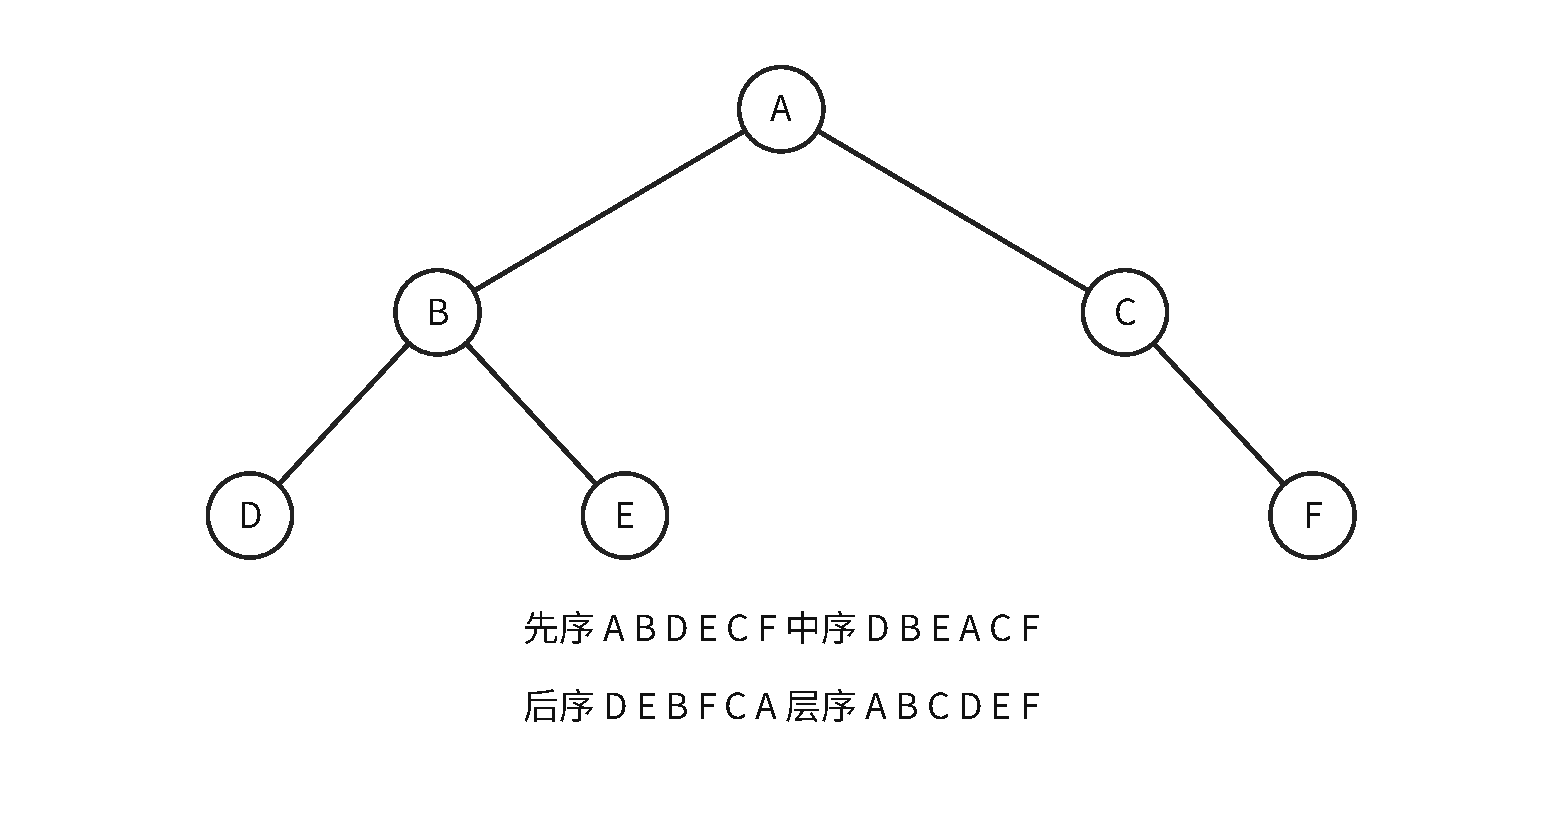
\includegraphics[width=\linewidth,height=125mm,keepaspectratio]{figures/DS_05_binary_traversal.pdf}
\captionof{figure}{同一棵二叉树的先中后序及层序；空的左孩子不应被当作另一个结点}\label{ds-fig-traversal}
\end{minipage}\par\medskip

先序为 \texttt{A B D E C F}；中序为 \texttt{D B E A C F}；后序为 \texttt{D E B F C A}；层序为 \texttt{A B C D E F}。先序在深入子树之前处理结点，适合复制或输出结构；后序在左右结果齐备后处理根，适合求子树大小、高度、释放结点。访问位置应服从依赖，不能只因为某种遍历最常见就选它。

\par\medskip\noindent\begin{minipage}{\linewidth}
\BlueLines{2,4}
\begin{codeblock}[language=C]
int TreeDepth(BiTree T) {
    if (T==NULL) return 0;
    int hl=TreeDepth(T->lchild), hr=TreeDepth(T->rchild);
    return 1+(hl>hr ? hl : hr);
}
\end{codeblock}
\end{minipage}\par\medskip

这段代码每个结点只处理一次，时间 \(O(n)\)；调用栈深为 \(O(h)\)。求高度时，叶结点返回1，与本章高度约定一致。交换所有左右子树可以递归地先交换两个子树内部，再交换两个孩子指针，从而把中序序列整体反向；交换不改变根的身份，也不改变哪些结点是叶结点。

课件中的另一棵树增加了D的右孩子G、C的左孩子F，可同时检查左右位置、访问时机与输出次序：

\par\medskip\noindent\begin{minipage}{\linewidth}
\centering
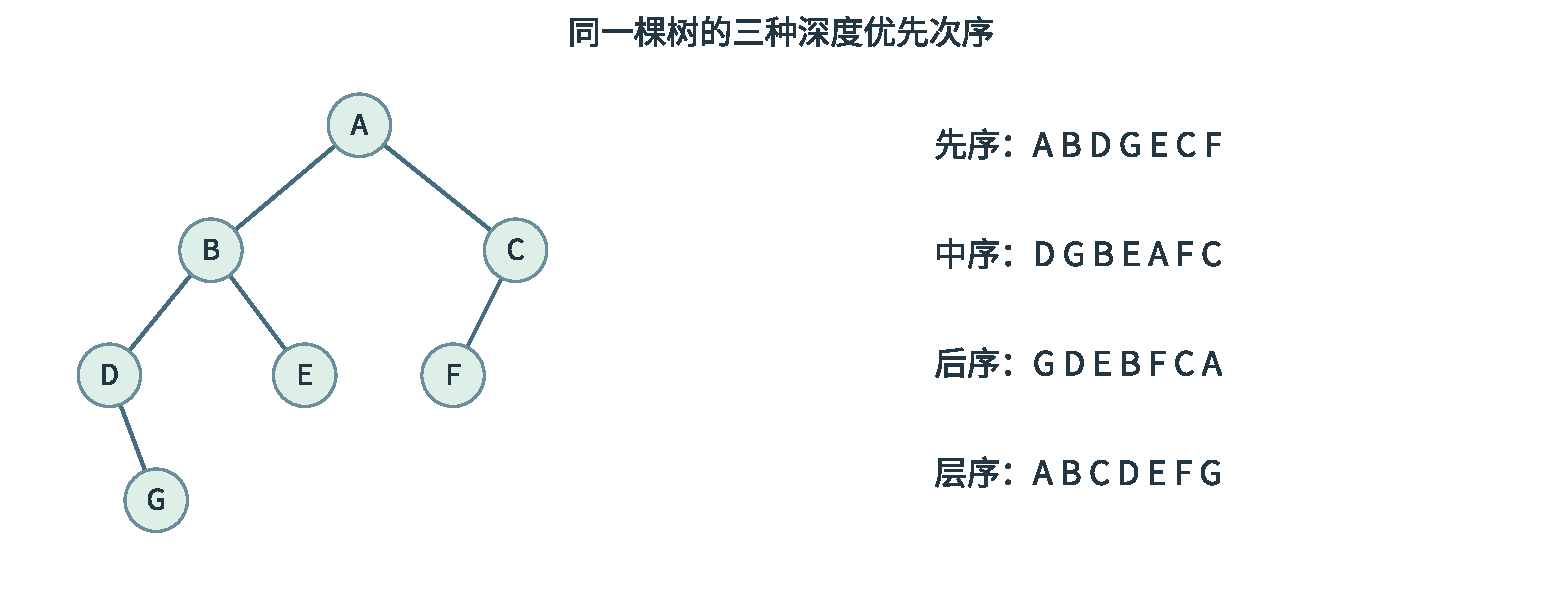
\includegraphics[width=\linewidth,height=125mm,keepaspectratio]{figures/DS05_lecture_traversal.pdf}
\captionof{figure}{原树与先序、中序、后序、层序的对应序列}\label{DS05-fig-lecture-traversal}
\end{minipage}\par\medskip

\subsection{递归遍历的三种访问位置}\label{DS05-order-code}

\par\medskip\noindent\begin{minipage}{\linewidth}
\BlueLines{2,9,16}
\begin{codeblock}[language=C++]
void PreOrder(BiTree T) {
    if (T!=NULL) {
        visit(T);
        PreOrder(T->lchild);
        PreOrder(T->rchild);
    }
}
void InOrder(BiTree T) {
    if (T!=NULL) {
        InOrder(T->lchild);
        visit(T);
        InOrder(T->rchild);
    }
}
void PostOrder(BiTree T) {
    if (T!=NULL) {
        PostOrder(T->lchild);
        PostOrder(T->rchild);
        visit(T);
    }
}
\end{codeblock}
\end{minipage}\par\medskip

把每个递归结点看成有三个停留点：进入左子树前、左子树返回后、右子树返回后。三种遍历仅改变\texttt{visit}所在停留点，递归下降和返回的骨架相同。时间都是\(\Theta(n)\)，最大同时存活的调用数由树高决定，辅助栈为\(O(h)\)；单支树可达\(O(n)\)，平衡形态为\(O(\log n)\)。表达式树的先序、后序分别产生前缀、后缀表达式；中序输出中缀表达式时要根据结构添加括号，才能保留原运算顺序。

\subsection{先序加中序为什么能还原}\label{ux5148ux5e8fux52a0ux4e2dux5e8fux4e3aux4ec0ux4e48ux80fdux8fd8ux539f}

假设结点标识互不相同。先序第一个元素为根，在中序中找到根后，左侧全属于左子树，右侧全属于右子树；由左子树的长度，能把先序余段分成左右两段，再递归。上图根为 A，中序左段 \texttt{D B E} 长3，故先序左段是 \texttt{B D E}，根B又把它分成D和E。

中序加后序也能唯一还原，根取后序最后一个；先序加后序一般不能区分一个单孩子在左还是在右。只给含 \(n\) 个不同标识的先序序列，形态数仍为卡特兰数 \(C_n\)，例如4个元素为14种。结点值重复时，``在中序中找到根的位置''可能不唯一，前述唯一性需要额外身份信息。

\subsection{由层序和中序还原}\label{DS05-rebuild}

结点标识互异时，层序首项是根；中序在根处分开左右子树。把其余层序项按``是否属于左侧中序集合''稳定筛分，得到左右子树各自的层序，再递归。

课件例：层序\texttt{A B C D E}、中序\texttt{A C B E D}。根为A，中序左侧为空，所以A没有左子树；右子树层序为\texttt{B C D E}，中序为\texttt{C B E D}。该子树根B，左子树只有C；右子树根D且左孩子为E。最终为\texttt{A(\allowbreak{}空,\allowbreak{}B(\allowbreak{}C,\allowbreak{}D(\allowbreak{}E,\allowbreak{}空)\allowbreak{})\allowbreak{})\allowbreak{}}。由此得到先序\texttt{A B C D E}、后序\texttt{C E D B A}。

课件另一组先序\texttt{D A E F B C H G I}、中序\texttt{E A F D H C B G I}，根D将中序分为\texttt{E A F}与\texttt{H C B G I}；左子树根A，孩子E、F；右子树根B，左子树为C且左孩子H，右子树根G且右孩子I。逐层分段比仅凭序列外观猜树形可靠。

\par\medskip\noindent\begin{minipage}{\linewidth}\fontsize{9.3}{12}\selectfont\begin{tabularx}{\linewidth}{@{}YYY@{}}
\toprule\noalign{}
已知序列，标识互异 & 一般能否唯一还原 & 决定子树范围的依据 \\
\midrule\noalign{}


先序＋中序 & 能 & 先序首项定根，中序分左右 \\
后序＋中序 & 能 & 后序末项定根，中序分左右 \\
层序＋中序 & 能 & 层序首项定根，中序分左右并筛层序 \\
先序＋后序 & 一般不能 & 单孩子的左右位置无法区分 \\
先序＋层序、后序＋层序 & 一般不能 & 两结点的单左、单右树即为反例 \\
\bottomrule\end{tabularx}
\end{minipage}\par\medskip

``需要中序''是一般二叉树、仅按这些遍历组合还原时的结论；增加满二叉树、显式空指针标记等约束后，要按新增信息重新分析。

非递归中序遍历用显式栈保存未完成的祖先：沿左链入栈，到空位置时弹栈访问，再转到其右子树。上图先依次压入 A、B、D，弹出 D 后没有右孩子，接着弹出 B 并转到 E；E 处理完才回到仍在栈中的 A。

\par\medskip\noindent\begin{minipage}{\linewidth}
\BlueLines{3,4}
\begin{codeblock}[language={}]
inorder(root):
    p=root; 建空栈 S
    while p 非空 or S 非空:
        while p 非空:
            push(S,p); p=p->lchild
        p=pop(S); visit(p)
        p=p->rchild
\end{codeblock}
\end{minipage}\par\medskip

非递归后序还需分辨右子树是否已经处理，可保存最近访问结点 \texttt{last}。从左子树返回时先看栈顶；它有尚未处理的右子树，就进入右子树，不能立即弹根。

\par\medskip\noindent\begin{minipage}{\linewidth}
\BlueLines{3,4,8}
\begin{codeblock}[language={}]
postorder(root):
    p=root; last=NULL; 建空栈 S
    while p 非空 or S 非空:
        if p 非空:
            push(S,p); p=p->lchild
        else:
            q=top(S)
            if q->rchild 非空 and last!=q->rchild:
                p=q->rchild
            else:
                visit(q); last=pop(S)
\end{codeblock}
\end{minipage}\par\medskip

\texttt{last} 只在一次完整子树处理后更新，因此它等于 \texttt{q->\allowbreak{}rchild}，表示右子树根已经最后访问过。每个结点各入栈、出栈一次，时间仍为 \(O(n)\)，栈最多同时保存一条祖先路径，空间为 \(O(h)\)。

层序遍历把根入队，反复出队访问并依次入队左右孩子。判定完全二叉树可在层序遍历中设置``已经遇到空孩子''标志：一旦出现空位置，此后的孩子位置不得再出现非空结点。只排除``有右孩子而无左孩子''还不够，还要排除遇到首个空孩子位置后又出现非空孩子的情况；一个结点只有左孩子，本身未必违反完全性。

\subsection{例 5-3　中序前驱和后继在哪一侧}\label{DS05-ex3}

\begin{example}[配套案例]

【配套例题】 p、q、v 都是二叉树 T 中的结点，v 有两个孩子，T 的中序遍历序列形如 \texttt{…,\allowbreak{}p,\allowbreak{}v,\allowbreak{}q,\allowbreak{}…}。正确的是（　）。

A. p没有右孩子，q没有左孩子　B. p没有右孩子，q有左孩子

C. p有右孩子，q没有左孩子　D. p有右孩子，q有左孩子

\end{example}

\textbf{解析。} v 有左子树，紧邻它之前的 p 必在左子树的最右端；若 p 还有右孩子，应先访问那棵右子树，p 就不可能紧邻 v。对称地，q 是右子树的最左端，不可能有左孩子。答案为 \textbf{A}。这里的``最右端''指沿右孩子指针一直走到不能再走的位置，不能按图上哪个结点画得最靠右来判断。

\begin{methodbox}[遍历问题先固定三个条件]

先写清访问根的位置、左右孩子顺序、空树处理。还原问题再检查结点身份是否唯一；若给先序与中序，根由先序首项决定，子树边界由中序决定，不能按数值大小猜左右。

\end{methodbox}

层序遍历的队列表示``已发现但尚未处理''的结点。以本章图为例，A出队后B、C入队，接着B出队才把D、E加入队尾，所以C在D之前处理。

\par\medskip\noindent\begin{minipage}{\linewidth}
\BlueLines{2,4,6}
\begin{codeblock}[language={}]
levelOrder(root):
    if root为空: return
    Q入队root
    while Q非空:
        p=Q出队; visit(p)
        if p.lchild非空: Q入队p.lchild
        if p.rchild非空: Q入队p.rchild
\end{codeblock}
\end{minipage}\par\medskip

时间\(O(n)\)；队列峰值由树的宽度决定，最坏\(O(n)\)。不能把递归遍历的\(O(h)\)调用栈结论搬到层序队列。

\section{线索二叉树：区分孩子链接与遍历线索}\label{DS05-05}

二叉链表有许多空孩子指针。把空左域改记某遍历次序下的前驱，把空右域改记后继，便得到相应的\textbf{线索二叉树}。新增 \texttt{ltag}、\texttt{rtag} 区分该域是孩子还是线索；本书约定0表示孩子，1表示线索。寻找子树时必须先看标志，不能沿一条线索继续递归，否则可能回到祖先形成循环。

中序线索树中，若结点右域为线索，可直接到中序后继；若右域为孩子，后继是右子树中沿真实左孩子链到达的第一个结点。前驱同理：左域为线索则直接取，否则到左子树最右端。图中每个结点的 L、R 分别表示左、右指针域，其后数字为对应的 \texttt{ltag}、\texttt{rtag}。E 的 R1 指向 A，C 的 L1 也指向 A；两条线索各有独立的起点和箭头落点。D 的 L1 和 F 的 R1 则分别接空前驱、空后继端点，本图采用无头结点、首尾取空的约定。

\par\medskip\noindent\begin{minipage}{\linewidth}
\centering
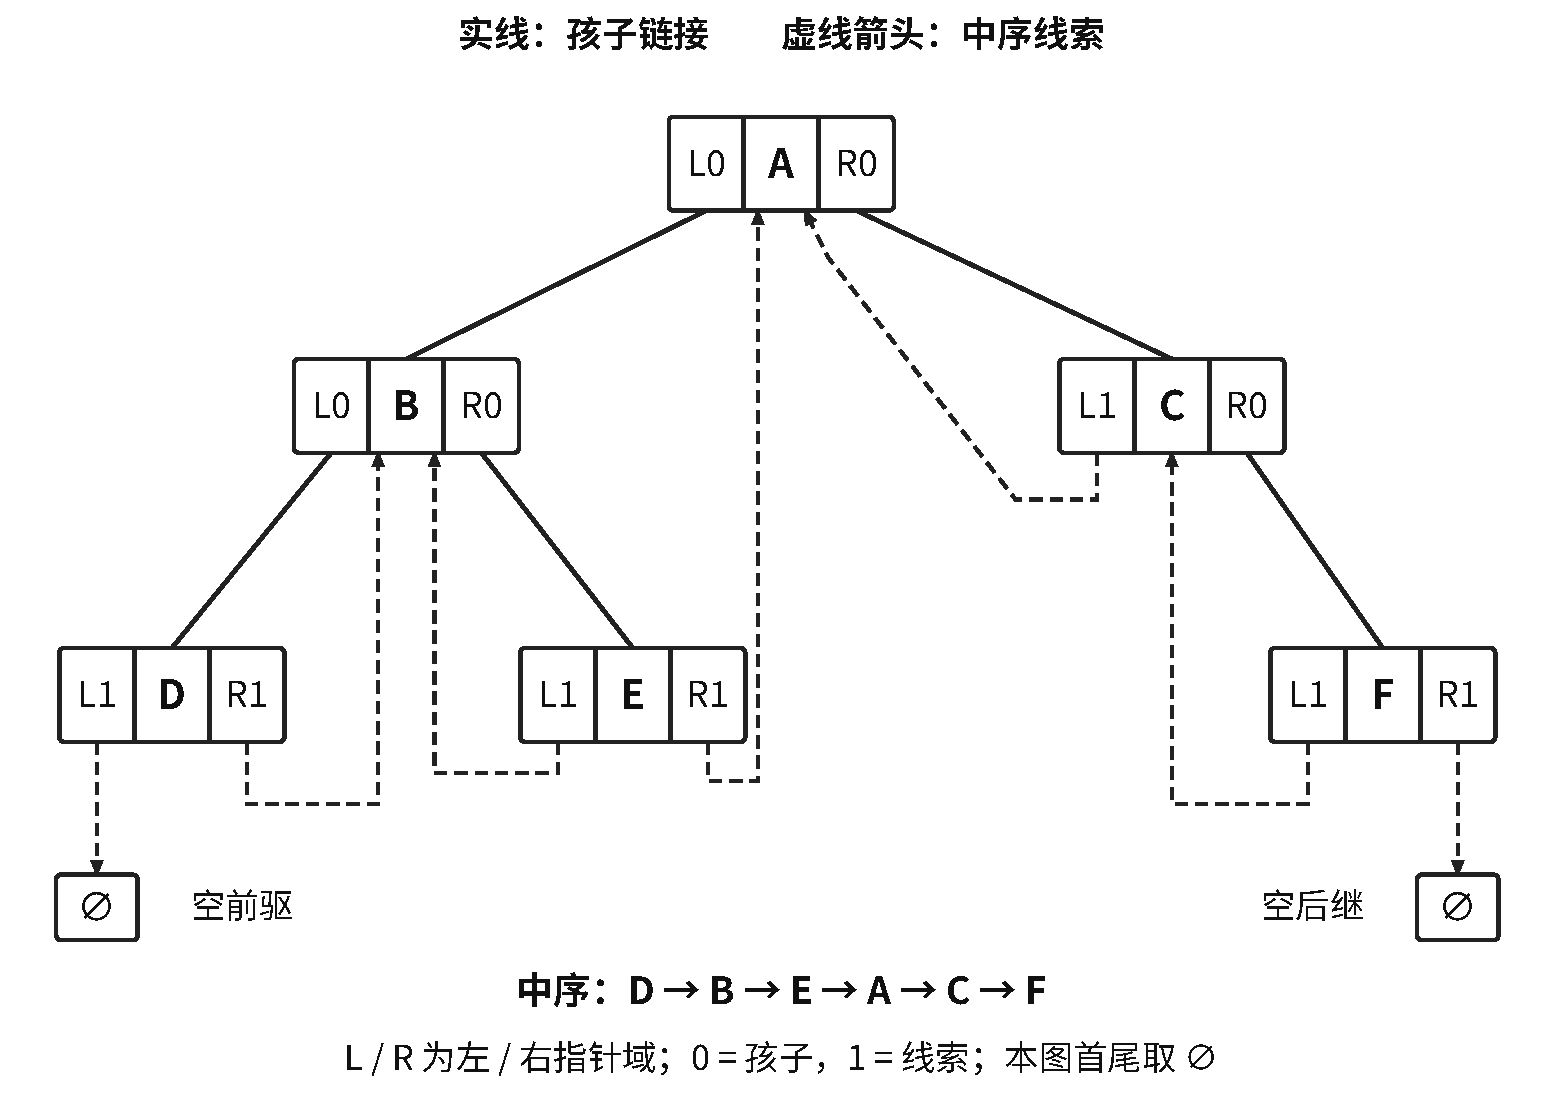
\includegraphics[width=\linewidth,height=125mm,keepaspectratio]{figures/DS_06_inorder_threads.pdf}
\captionof{figure}{虚线为中序线索，实线为孩子；首尾边界单独标出}\label{ds-fig-threads}
\end{minipage}\par\medskip

\(n+1\) 个原空孩子域均可改为线索域，其中首结点的前驱和末结点的后继需约定为空或指向专设头结点。题目说``线索数为 \(n+1\)''时通常统计这些线索域，包含首尾边界；若只统计实际指向普通结点的线索，则边界两项另算。加头结点后，其额外指针也不应混入原树的 \(2n\) 域计数。

构造中序线索时，用 \texttt{pre} 保存刚访问过的结点，初值为空。处理当前结点p时，若其左域为空，填入pre并设置左线索标志；若pre的右域为空，填入p并设置右线索标志，随后令pre=p。递归只沿真实孩子执行，避免把刚填的线索又当作子树。

\par\medskip\noindent\begin{minipage}{\linewidth}
\BlueLines{8,10,14}
\begin{codeblock}[language=C++]
typedef struct ThreadNode {
    ElemType data;
    struct ThreadNode *lchild, *rchild;
    int ltag, rtag;  // 0：孩子；1：线索
} ThreadNode, *ThreadTree;

void InThread(ThreadTree p, ThreadTree &pre) {
    if (p!=NULL) {
        InThread(p->lchild, pre);
        if (p->lchild==NULL) {
            p->lchild=pre;
            p->ltag=1;
        }
        if (pre!=NULL && pre->rchild==NULL) {
            pre->rchild=p;
            pre->rtag=1;
        }
        pre=p;
        InThread(p->rchild, pre);
    }
}
void CreateInThread(ThreadTree T) {
    ThreadTree pre=NULL;
    if (T!=NULL) {
        InThread(T, pre);
        pre->rchild=NULL;
        pre->rtag=1;
    }
}
\end{codeblock}
\end{minipage}\par\medskip

调用前所有原孩子标志为0。图中先访问D，其空左域指向空前驱；随后访问B，D的空右域才补为指向B的线索。访问E时填左线索指向B，访问A时再把E的空右域补为A。遍历结束后，pre为最后结点F，将其空右域标为后继线索，线索目标按约定为空或为头结点。若使用头结点，首结点空前驱也应统一改指头结点。

先序、后序线索的前驱后继依照各自次序，不可沿用中序规则。后序中，若叶结点 X 存在左兄弟 Y，则 X 是双亲的右孩子；左子树和右子树都处理完后才访问双亲，因此 X 的后序后继是双亲，而不是左兄弟。一般后序线索树若无双亲信息，不一定能像中序那样方便地只凭孩子和线索完成全部后继访问。

\subsection{线索树的访问算法与六种前驱后继}\label{DS05-thread-access}

\texttt{pre}以引用传入，使左子树递归更新后的``刚访问结点''能够传回当前层；若按值传指针，调用返回后当前层仍拿着旧值。教材中序线索化只对原始、标志均为0的二叉链表调用。右递归开始前，当前结点原本非空的右孩子未被改写；因此该版本可直接递归右孩子。再次对已线索化的树调用时，必须按标志辨别真实孩子。

\par\medskip\noindent\begin{minipage}{\linewidth}
\BlueLines{2,3,6}
\begin{codeblock}[language=C++]
ThreadNode *Firstnode(ThreadNode *p) {
    while (p->ltag==0) p=p->lchild;
    return p;
}
ThreadNode *Nextnode(ThreadNode *p) {
    if (p->rtag==0) return Firstnode(p->rchild);
    return p->rchild;
}
void InOrderThread(ThreadNode *T) {
    if (T==NULL) return;
    for (ThreadNode *p=Firstnode(T); p!=NULL; p=Nextnode(p))
        visit(p);
}
\end{codeblock}
\end{minipage}\par\medskip

\texttt{Firstnode}的前提是参数非空、所有空左域均已正确标成线索；\texttt{Nextnode}接收一个实际结点。这样无需递归栈即可中序遍历。找一次后继最坏可能沿一条左链，整趟遍历每条孩子链接只走常数次，故总时间\(O(n)\)、额外空间\(O(1)\)。

\par\medskip\noindent\begin{minipage}{\linewidth}\fontsize{9.3}{12}\selectfont\begin{tabularx}{\linewidth}{@{}YYY@{}}
\toprule\noalign{}
\begin{minipage}[b]{\linewidth}\raggedright
线索类型
\end{minipage} & \begin{minipage}[b]{\linewidth}\raggedright
找前驱
\end{minipage} & \begin{minipage}[b]{\linewidth}\raggedright
找后继
\end{minipage} \\
\midrule\noalign{}


中序 & 左域为线索则直接取；否则左子树最右结点 & 右域为线索则直接取；否则右子树最左结点 \\
先序 & 左域为线索则直接取；有左孩子时通常还需双亲信息 & 有左孩子先取左孩子，否则取右域（孩子或线索） \\
后序 & 有右孩子先取右孩子，否则取左域（孩子或线索） & 右域为线索则直接取；有右孩子时通常还需双亲信息 \\
\bottomrule\end{tabularx}
\end{minipage}\par\medskip

先序有左孩子的结点，其前驱在子树之外；后序有右孩子的结点，其后继在子树之外，因此普通二叉线索链表未必能直接取得。若有双亲域：先序中，左孩子的前驱是双亲；右孩子无左兄弟时前驱是双亲，有左兄弟时为左兄弟子树最后一个先序结点。后序对称：右孩子的后继是双亲，左孩子无右兄弟时后继是双亲，有右兄弟时为右兄弟子树第一个后序结点。

先序线索化在访问根后才递归，刚建立的左线索可能指回祖先，故递归左侧必须检查\texttt{ltag=\allowbreak{}=\allowbreak{}0}。后序先完成两棵原子树再建线索，注意结束后末结点是根，根未必原本没有右孩子；处理收尾时应判断空右域，不能照搬中序``最后结点右孩子必空''的条件。

\section{普通树的三种存储}\label{DS05-06}

\textbf{双亲表示法}为每个结点保存双亲的下标，根用 \ensuremath{-}1 等特殊值标识。找双亲 \(O(1)\)，找全部孩子通常需扫描整个数组。它适合从结点反复向根追踪，却不便于列举孩子。

\textbf{孩子表示法}为每个结点保存孩子链表，便于依次访问所有孩子；反查双亲时若没有另外保存双亲信息，仍需搜索。\textbf{孩子兄弟表示法}只保存两个链接：\texttt{firstChild} 指向第一个孩子，\texttt{nextSibling} 指向下一个兄弟。它能用两个指针表示孩子数不定的树，却不能把 \texttt{nextSibling} 理解成普通树的孩子。

选择表示时，应先看主要方向：查双亲、枚举孩子或遍历同层兄弟，分别依赖不同的链接。多保存一个双亲域会增加空间，但上溯不必再搜索，代价降低。

\subsection{三种树存储的教材结构}\label{DS05-tree-storage-code}

\par\medskip\noindent\begin{minipage}{\linewidth}
\begin{codeblock}[language=C++]
#define MAX_TREE_SIZE 100
typedef struct {
    ElemType data;
    int parent;
} PTNode;
typedef struct {
    PTNode nodes[MAX_TREE_SIZE];
    int n;
} PTree;

typedef struct CSNode {
    ElemType data;
    struct CSNode *firstchild, *nextsibling;
} CSNode, *CSTree;
\end{codeblock}
\end{minipage}\par\medskip

双亲数组中根的\texttt{parent=\allowbreak{}-1}，其余值为双亲在数组中的下标，不能把它当作元素数据。孩子表示法则在顺序顶点表的每个元素中保存孩子链首指针，链结点保存孩子下标和下一孩子指针；它是顺序与链式存储的结合。森林的双亲表示可有多个\texttt{parent=\allowbreak{}-1}，孩子表示则须保存各根的位置。孩子兄弟表示中，森林各根沿\texttt{nextsibling}相连。

\section{树、森林怎样转换为二叉树}\label{DS05-07}

采用``左孩子、右兄弟''约定：普通树第一个孩子成为二叉树左孩子，后续兄弟依次以右孩子相连。原树的根没有兄弟，故其对应二叉树的根没有右孩子。森林的各棵树根互为兄弟，再沿右链连接，第一棵树的根成为二叉树的根。

\par\medskip\noindent\begin{minipage}{\linewidth}
\centering
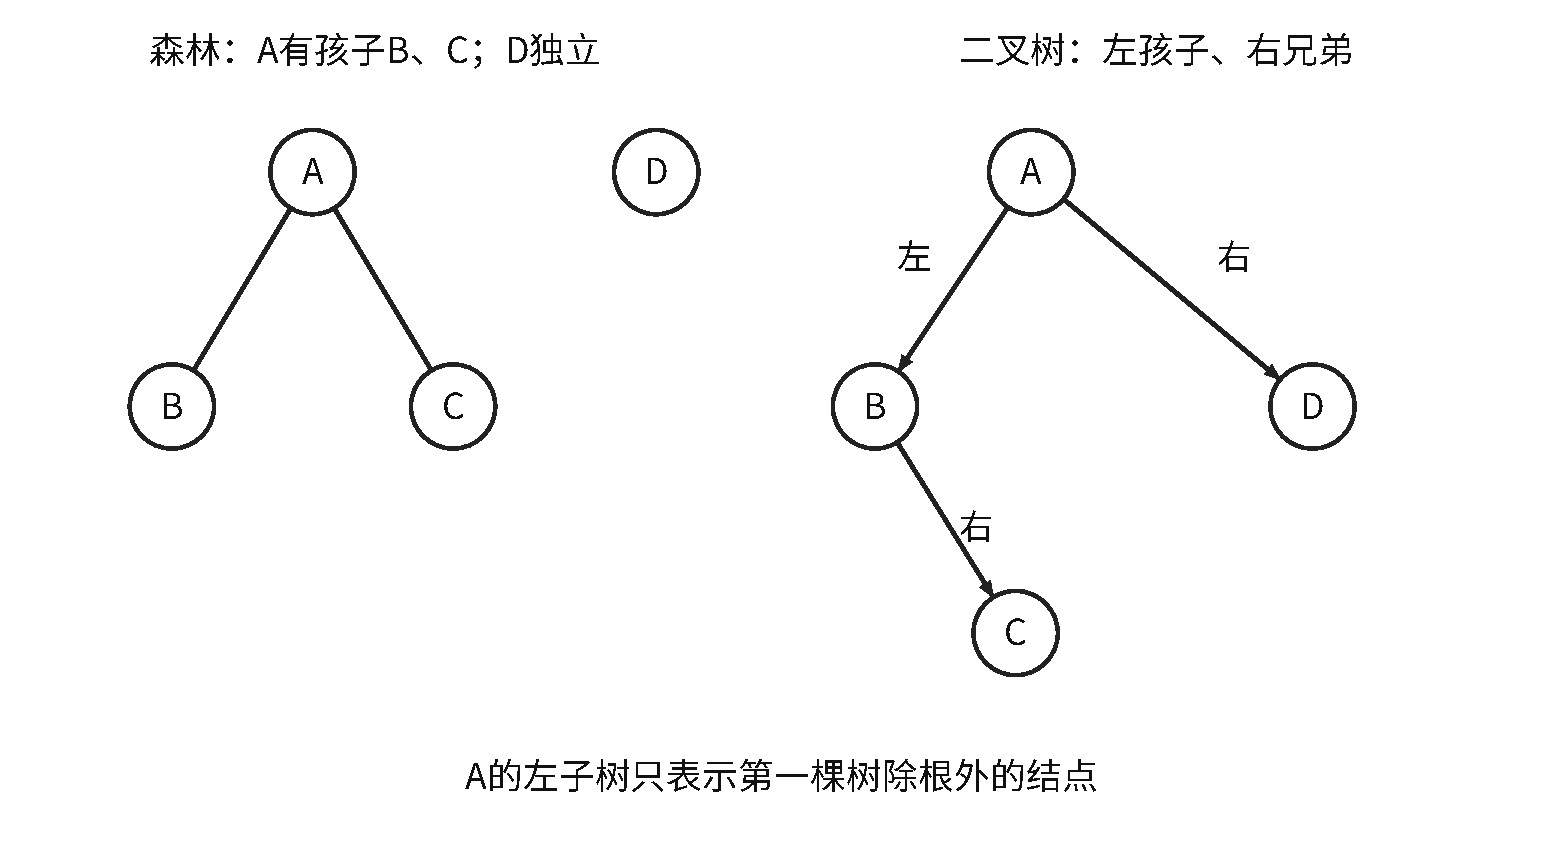
\includegraphics[width=\linewidth,height=125mm,keepaspectratio]{figures/DS_07_forest_conversion.pdf}
\captionof{figure}{普通树的孩子关系转成左孩子，兄弟关系转成右孩子}\label{ds-fig-forest}
\end{minipage}\par\medskip

逆转换时，从某结点的左孩子出发沿右链走，沿途结点就是它的全部孩子；根及其右链上的各结点分别作为森林各棵树的根。转换改变了``左右链接的解释''，没有增加或删除数据结点。森林有4棵树、第一棵含 \(a\) 个结点时，二叉树根的左子树只含第一棵树除根外的 \(a-1\) 个结点，其他树由根的右子树表示。

\subsection{例 5-4　二叉树隔两条链接，在森林中是什么关系}\label{DS05-ex4}

\begin{example}[配套案例]

【配套例题】 将森林转换成对应二叉树。若二叉树中 u 是 v 的父结点的父结点，则原森林中 u 与 v 可能的关系是（　）。

\ensuremath{\mathrm{I}}. 父子关系　\ensuremath{\mathrm{II}}. 兄弟关系　\ensuremath{\mathrm{III}}. u 的父结点与 v 的父结点是兄弟关系

A. 只有\ensuremath{\mathrm{II}}　B. \ensuremath{\mathrm{I}}和\ensuremath{\mathrm{II}}　C. \ensuremath{\mathrm{I}}和\ensuremath{\mathrm{III}}　D. \ensuremath{\mathrm{I}}、\ensuremath{\mathrm{II}}和\ensuremath{\mathrm{III}}

\end{example}

\textbf{解析。} 从 u 到 v 恰经过两条二叉树链接。左---右表示``先到 u 的第一个孩子，再到其下一个兄弟''，v 仍是 u 的孩子，\ensuremath{\mathrm{I}}可能；右—右表示连续两个兄弟链接，u、v 互为兄弟，\ensuremath{\mathrm{II}}可能。左—左表示祖孙，右—左表示 u 的兄弟的孩子，它们都不能产生\ensuremath{\mathrm{III}}所说的父结点关系。因此答案为 \textbf{B}。应按每条链接的语义推回森林，不能把二叉树的双亲直接当作原树的双亲。

\section{树与森林的遍历怎样对应}\label{DS05-08}

普通树的先根遍历先访问根，再依次先根遍历各子树；后根遍历先按顺序遍历各子树，再访问根。采用孩子兄弟转换后，树的先根次序对应二叉树先序，树的后根次序对应二叉树中序。原因是二叉树左链接深入第一个孩子，而右链接串联后续兄弟。

森林先序依次先根遍历各棵树，对应二叉树先序；森林中序先按中序处理第一棵树的子树森林，再访问该树根，最后处理其余树，对应二叉树中序。森林遍历要按定义递归到各棵树，并非在整片森林开头统一访问一次根。

层次遍历普通树时，出队一个结点后，按孩子链的次序把它的所有孩子入队；兄弟链接只用于枚举孩子，不能把整条兄弟链当成下一层的结点序列。

\section{哈夫曼树、WPL 与前缀编码}\label{DS05-09}

给每个叶结点一个权值 \(w_i\)，根到它的路径长度（边数）为 \(d_i\)，\textbf{带权路径长度}为 \(\mathrm{WPL}=\sum_iw_id_i\)。权值通常为频数或概率，内部结点不直接加入这项``叶权乘深度''的求和。求给定叶权下最小 WPL 的二叉树，可每次选当前两个最小权值合并为新结点，再把权值和放回候选集合，直到仅剩根。

为什么合并两个最小值：在一棵最优树中，可以让最深的一对兄弟叶承载两个最小权值而不增大 WPL；把它们收缩成一个权值为和的叶后，剩余结构仍应最优，否则替换后能得到 WPL 更小的树。每次合并都使这两棵子树中所有叶的深度增加1，因此合并权值之和也等于最终 WPL。

\subsection{例 5-5　加权平均码长怎样从合并过程得到}\label{DS05-ex5}

\begin{example}[配套案例]

【配套例题】 6个字符出现频次分别为3、4、5、6、8、10，为它们构造哈夫曼编码，加权平均长度为（　）。

A. 2.4　B. 2.5　C. 2.67　D. 2.75

\end{example}

\textbf{解析。} 每轮重新从当前候选中取最小的两个，不能把原始序列分成相邻对后一次配完。

\begin{wideblock}

\par\medskip\noindent\begin{minipage}{\linewidth}\fontsize{9.3}{12}\selectfont\begin{tabularx}{\linewidth}{@{}YYY@{}}
\toprule\noalign{}
本轮合并 & 新权值 & 合并后候选权值 \\
\midrule\noalign{}


3与4 & 7 & 5、6、7、8、10 \\
5与6 & 11 & 7、8、10、11 \\
7与8 & 15 & 10、11、15 \\
10与11 & 21 & 15、21 \\
15与21 & 36 & 36 \\
\bottomrule\end{tabularx}
\end{minipage}\par\medskip

\end{wideblock}

WPL 为 \(7+11+15+21+36=90\)，频次总和36，所以平均码长为 \(90/36=2.5\) 位/字符，答案为 \textbf{B}。不能把总码长除以6，因为各字符出现频次不同。

\par\medskip\noindent\begin{minipage}{\linewidth}
\centering
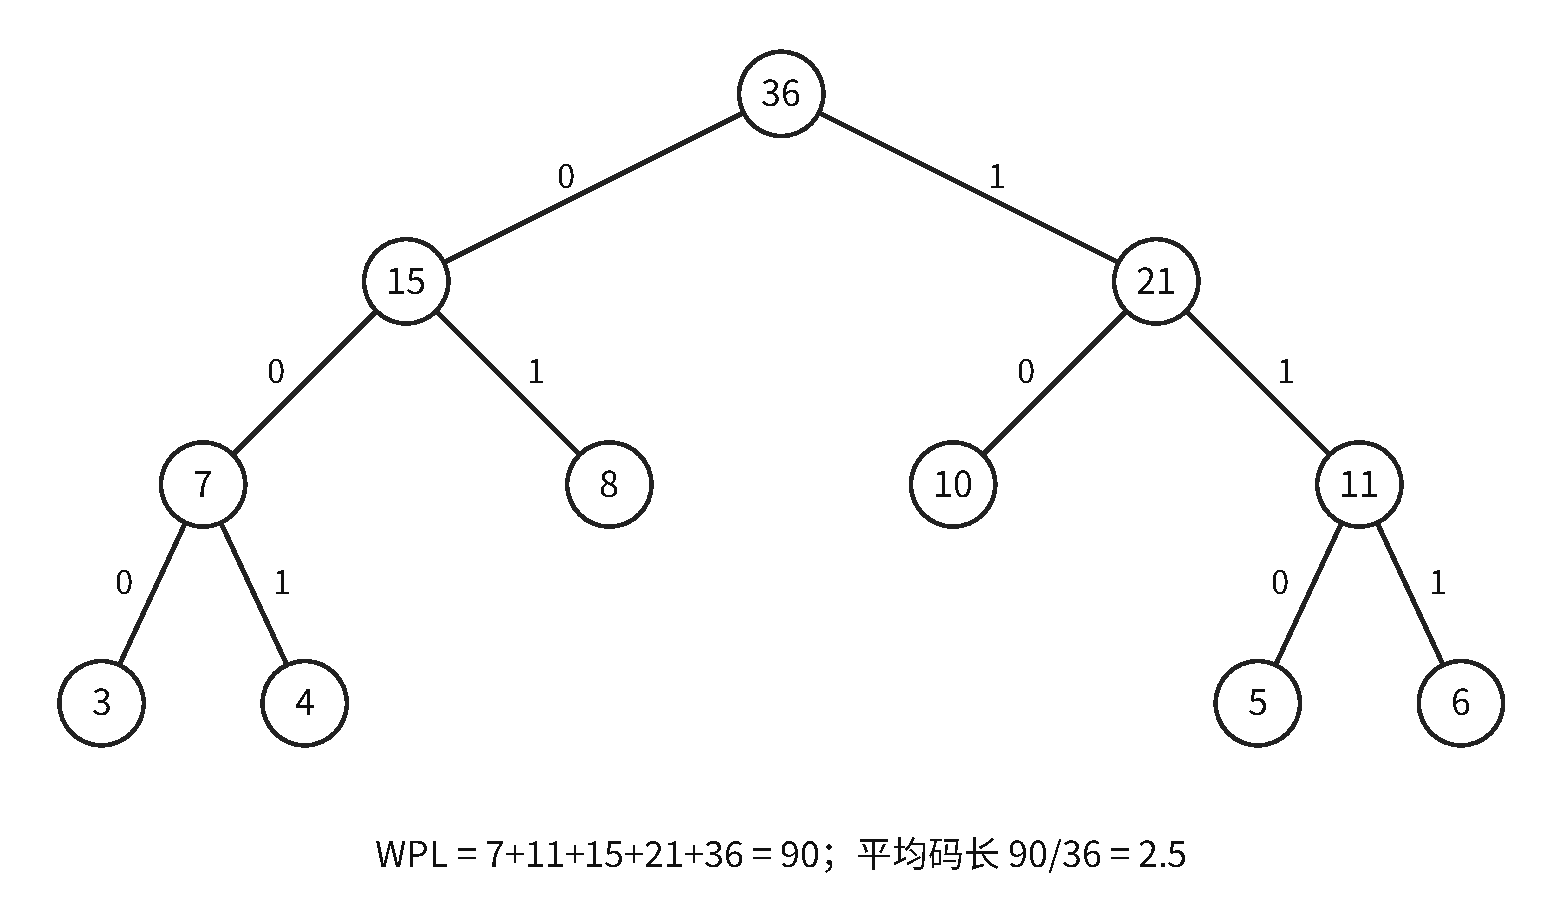
\includegraphics[width=\linewidth,height=125mm,keepaspectratio]{figures/DS_08_huffman.pdf}
\captionof{figure}{同一合并过程构造的哈夫曼树；左右分支的 0、1 可对换}\label{ds-fig-huffman}
\end{minipage}\par\medskip

沿根到叶的0、1路径形成码字。字符只放在叶上，所以任何字符码都不是另一个字符码的前缀，这称为\textbf{前缀编码}。编码可因相等权值的选取、左右分支交换而不唯一，WPL 仍可相同。哈夫曼树没有度为1的内部结点，若有 \(n\) 个叶，内部结点 \(n-1\)、总结点 \(2n-1\)；它未必完全、未必平衡，\(n\) 个叶的最大高度可达 \(n\)。

\subsection{王道课件中的合并与压缩实例}\label{DS05-huffman-course}

权值为\texttt{1,\allowbreak{}3,\allowbreak{}2,\allowbreak{}2,\allowbreak{}7}时，取相等权值的一种合法顺序：先合并1与2得到3，再将另一个2与新3合为5，原3与5合为8，最后7与8合为15。WPL等于全部合并权值之和：\(3+5+8+15=31\)。权相等时可以换选，形态和码字可能变化，最优WPL保持31。

再看课件的100题答案：C、A、B、D分别出现80、10、8、2次。固定2位编码共需200 bit；哈夫曼合并为\(2+8=10\)、\(10+10=20\)、\(20+80=100\)，WPL为\(10+20+100=130\) bit。按图中左0右1，可取C为0、A为10、D为110、B为111，平均码长\(130/100=1.3\) bit/题。与固定2位相比，编码数据长度为原来的65\%，节省35\%；这里暂未计入传递码表等附加信息。

\par\medskip\noindent\begin{minipage}{\linewidth}
\centering
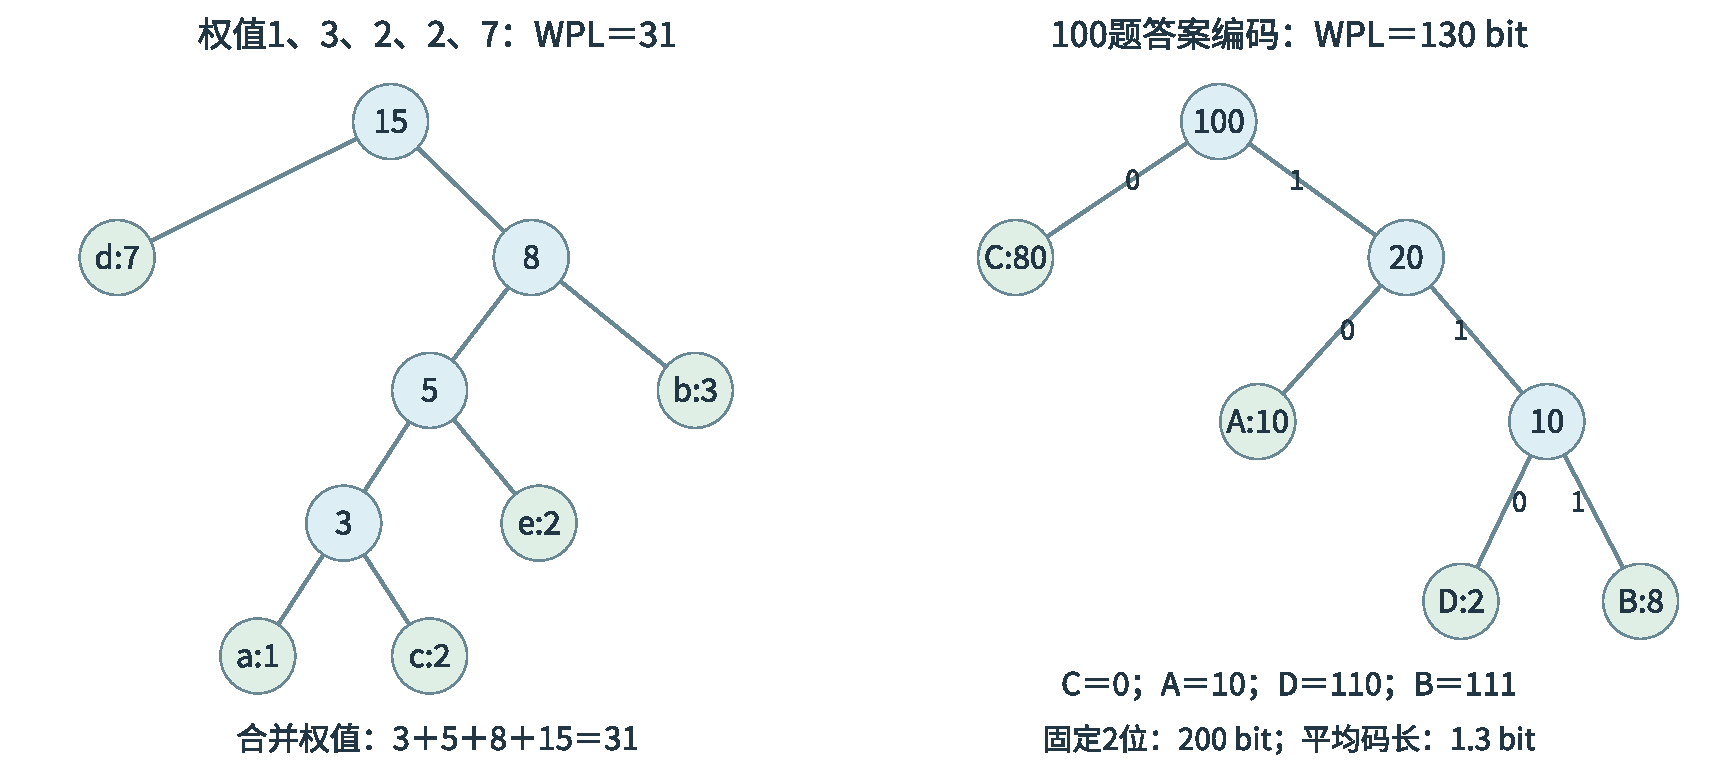
\includegraphics[width=\linewidth,height=125mm,keepaspectratio]{figures/DS05_huffman_course.pdf}
\captionof{figure}{两组王道课件数据的哈夫曼树、合并权值与码字}\label{DS05-fig-huffman-course}
\end{minipage}\par\medskip

例如\texttt{CAAABD}编码为\texttt{0|10|10|10|111|110}。沿树由根读取比特，到叶即输出一个字符再回根，就能解出原串；每个字符在叶上，因此完整码字不会是另一完整码字的前缀。

\subsection{例 5-6　已占用的码字怎样限制剩余容量}\label{DS05-ex6}

\begin{example}[配套案例]

〖5.5-004〗 哈夫曼编码长度不超过4，已有两个字符编码为1和01，还最多能对几个字符编码？

A. 2　B. 3　C. 4　D. 5

\end{example}

\textbf{解析。} 以1开头的整棵子树已被码字1占用，以01开头的子树也被占用。剩余码字只能位于00开头的子树。长度至多4，00之后最多还放2位，最多形成 \texttt{0000、0001、0010、0011} 四个叶，答案为 \textbf{C}。使用较短的剩余码会占用其后代位置，不会增加字符总数。

推广到 \(m\) 叉最优归并/编码时，每次合并最小的 \(m\) 个权值。若叶数不满足满 \(m\) 叉树的条件 \((n-1)\bmod(m-1)=0\)，可补最少的零权虚叶。补齐后的叶数记 \(n'\)，内部结点数为 \((n'-1)/(m-1)=\lceil(n-1)/(m-1)\rceil\)；不能直接把二叉的``内部结点 \(n-1\)''照搬。这里内部结点都按m叉合并计算，零权虚叶不代表额外字符。第8章最佳归并树会再次使用这项结构关系。

\begin{methodbox}[把哈夫曼的贪心选择写成可重复步骤]

候选森林初始为各带权叶；重复取两个最小权根，创建权值为两者之和的新根，并将它放回候选集合。每轮候选数减少1，故\(n\)个符号需\(n-1\)轮。优先队列实现总时间\(O(n\log n)\)，树与候选存储\(O(n)\)；单符号编码的码长需另作约定。

\end{methodbox}

\par\medskip\noindent\begin{minipage}{\linewidth}
\BlueLines{3,7}
\begin{codeblock}[language={}]
huffman(weights):
    Q=以权值为键的小根优先队列
    while size(Q)>1:
        a=extractMin(Q); b=extractMin(Q)
        z=new Node(weight=a.weight+b.weight,left=a,right=b)
        insert(Q,z)
    return Q唯一根（若原输入为空则返回空）
\end{codeblock}
\end{minipage}\par\medskip

\section{并查集：用根结点代表一个集合}\label{DS05-10}

并查集维护若干互不相交的集合，主要支持两个操作：\texttt{find(\allowbreak{}x)\allowbreak{}} 查 x 所在集合的代表元，\texttt{union(\allowbreak{}x,\allowbreak{}y)\allowbreak{}} 合并两个集合。它不要求维护集合内部元素的顺序。用数组 \texttt{parent} 表示一片双亲森林，根存负数表示集合规模，非根存双亲下标。

例如初始6个单元素集合：\texttt{parent=\allowbreak{}[\allowbreak{}−1,\allowbreak{}−1,\allowbreak{}−1,\allowbreak{}−1,\allowbreak{}−1,\allowbreak{}−1]\allowbreak{}}。合并0与1后可记 \texttt{parent[\allowbreak{}0]\allowbreak{}=\allowbreak{}−2,\allowbreak{}parent[\allowbreak{}1]\allowbreak{}=\allowbreak{}0}；再合并2与3得 \texttt{parent[\allowbreak{}2]\allowbreak{}=\allowbreak{}−2,\allowbreak{}parent[\allowbreak{}3]\allowbreak{}=\allowbreak{}2}；把这两集合合并时，把根2接到根0，根0规模记\ensuremath{-}4。查找3时沿3\ensuremath{\to}2\ensuremath{\to}0，不能把直接双亲2误当作最终代表。

\textbf{按规模合并}让较小树根接到较大树根，避免不断形成长链；\textbf{路径压缩}在查找后把沿途结点直接连到根。路径压缩不改变集合划分，只改变表示。两项同时使用时，连续操作的摊还复杂度极低，可用反阿克曼函数表示；单次查找仍须按当时实际路径执行，不能声称每次严格只访问一个结点。

\par\medskip\noindent\begin{minipage}{\linewidth}
\BlueLines{5,6,9}
\begin{codeblock}[language=C++]
void Initial(int S[], int n) {
    for (int i=0; i<n; ++i) S[i]=-1;
}
int Find(int S[], int x) {
    while (S[x]>=0) x=S[x];
    return x;
}
void Union(int S[], int Root1, int Root2) {
    if (Root1==Root2) return;
    S[Root2]=Root1;
}
\end{codeblock}
\end{minipage}\par\medskip

这里的\texttt{Union}参数是两个\textbf{根下标}，调用前应先\texttt{Find}。基础版本中根的负值只作根标志，合并时不维护规模。若使用按规模优化，则根负值必须始终等于负的结点总数，两种实现不能交叉调用。

\par\medskip\noindent\begin{minipage}{\linewidth}
\BlueLines{2,3,13}
\begin{codeblock}[language=C++]
void UnionBySize(int S[], int Root1, int Root2) {
    if (Root1==Root2) return;
    if (S[Root2]>S[Root1]) {
        S[Root1]+=S[Root2];
        S[Root2]=Root1;
    } else {
        S[Root2]+=S[Root1];
        S[Root1]=Root2;
    }
}
int FindCompress(int S[], int x) {
    int root=x;
    while (S[root]>=0) root=S[root];
    while (x!=root) {
        int t=S[x];
        S[x]=root;
        x=t;
    }
    return root;
}
\end{codeblock}
\end{minipage}\par\medskip

按规模合并使较小树结点每上升一层，其所属集合规模至少加倍，树高至多\(\lfloor\log_2 n\rfloor+1\)。路径压缩和按规模合并同时使用时，\(m\)次操作的总开销可写为\(O(m\alpha(n))\)，这是摊还界；不能把它改说成任意一棵当前树高度严格等于\(\alpha(n)\)。

Kruskal 选边时，若两个端点代表元相同，加边会在现有森林中形成环；代表元不同才合并。这里代表的是当前已选边连成的分量，不是原图预先固定的一个编号。

\section{堆的结构、调整与优先队列}\label{DS05-11}

\textbf{二叉堆}同时满足完全二叉树的形状和堆序。大根堆中每个双亲关键字不小于孩子，小根堆中不大于孩子。于是根保存全局最大值或最小值；兄弟间没有规定，整个数组也不必有序。堆中沿根到叶的关键字单调，二叉搜索树则按左右子树区间有序，二者不是同一个约束。

本书堆用下标从1开始的数组。小根堆的最大值一定可以在叶中找到，叶下标为 \(\lfloor n/2\rfloor+1\sim n\)；不能确定是哪一个叶。非根结点若比所有后代都小，仍不保证它比别的子树中的元素小。

插入时先放到数组末尾，保证完全性，再与双亲比较并向上调整。删除根时，用末元素填根、缩小堆范围，再从根向下调整：选择较优孩子，与待调整的值比较，必要时交换并继续。每次最多跨越树高，时间 \(O(\log n)\)。原有左右子树必须已是堆，下滤才只需沿一条路径。

\par\medskip\noindent\begin{minipage}{\linewidth}
\centering
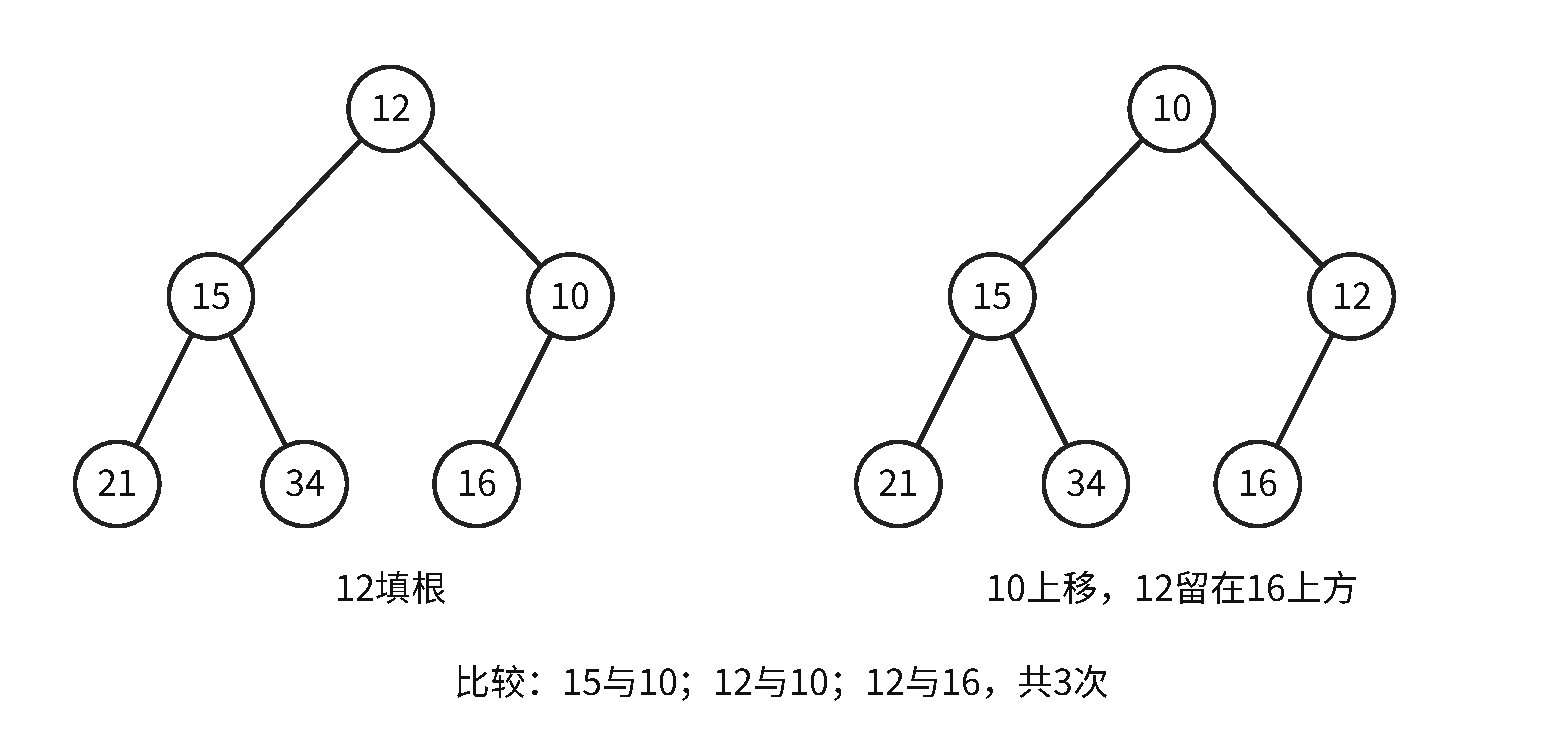
\includegraphics[width=\linewidth,height=125mm,keepaspectratio]{figures/DS_09_heap_delete.pdf}
\captionof{figure}{小根堆删根后，用末元素12填根，再与更小孩子10比较并下滤}\label{ds-fig-heap}
\end{minipage}\par\medskip

建堆从最后一个非叶结点 \(\lfloor n/2\rfloor\) 开始逆序下滤。叶子本身已是堆，靠下的内部结点移动距离短；按各高度结点数求和，建堆总时间为 \(O(n)\)，不是把每个结点都按最坏树高估成 \(O(n\log n)\)。逐个插入也能建堆，但对应另一种过程和复杂度上界。第8章将用同一调整规则执行完整堆排序。

\subsection{堆下滤的代码与不变式}\label{DS05-sift}

以下大根堆采用1起始数组。调用前，左右子树各自满足堆序，只可能根位置过小；每轮把较大孩子提升，尚未解决的缺口沿一条链向下移动。

\par\medskip\noindent\begin{minipage}{\linewidth}
\BlueLines{4,5}
\begin{codeblock}[language=C++]
void HeadAdjust(int A[], int k, int len) {
    A[0]=A[k];
    for (int i=2*k; i<=len; i*=2) {
        if (i<len && A[i]<A[i+1]) ++i;
        if (A[0]>=A[i]) break;
        A[k]=A[i]; k=i;
    }
    A[k]=A[0];
}
\end{codeblock}
\end{minipage}\par\medskip

向下每轮至少下降一层，最坏\(O(\log n)\)，辅助\(O(1)\)。只比较候选与左孩子会漏掉更大的右孩子；\texttt{i<\allowbreak{}len}是检查右孩子确实存在。空堆不应调用此函数，外部循环从\(n/2\)开始可自然跳过\(n=0,1\)的情况。

\begin{wideblock}

\par\medskip\noindent\begin{minipage}{\linewidth}\fontsize{9.3}{12}\selectfont\begin{tabularx}{\linewidth}{@{}YYY@{}}
\toprule\noalign{}
结构 & 约束保存什么 & 操作与判断边界 \\
\midrule\noalign{}


普通二叉树 & 左右位置有别 & 遍历还原需序列与身份条件 \\
完全二叉树 & 编号占据前\(n\)个位置 & 适合数组；只排除右孩子孤立还不够 \\
二叉堆 & 完全形状及双亲孩子间堆序 & 根为最值；兄弟不保证有序 \\
BST（第7章） & 全部左右子树的关键字区间 & 中序有序；不保证完全或平衡 \\
哈夫曼树 & 叶权下的WPL最小 & 通常不是完全树；编码可不唯一 \\
\bottomrule\end{tabularx}
\end{minipage}\par\medskip

\end{wideblock}

\section{主动回忆自测}\label{DS05-check}

以下为自拟补充，针对表示与前置条件。

\begin{enumerate}
\def\labelenumi{\arabic{enumi}.}
\item
  一棵二叉树有8个度为2的结点、3个度为1的结点，共多少结点？它是否一定为完全二叉树？
\item
  一棵二叉树的先序和中序完全相同，结点值互异，所有非叶结点的孩子位置有什么限制？
\item
  并查集中 \texttt{parent[\allowbreak{}4]\allowbreak{}=\allowbreak{}2,\allowbreak{}parent[\allowbreak{}2]\allowbreak{}=\allowbreak{}0,\allowbreak{}parent[\allowbreak{}0]\allowbreak{}=\allowbreak{}−5}，执行带路径压缩的 \texttt{find(\allowbreak{}4)\allowbreak{}} 后，哪些关系改变？
\item
  关键字互不相同的大根堆中，第二大元素一定在哪些可能位置？
\item
  为什么一棵\(n\)结点二叉链表有\(n+1\)个空孩子域？加上双亲域后怎样变化？
\item
  普通树的后根遍历转换后对应二叉树哪一种遍历？为什么不是后序？
\item
  权值3、4、5合并构造哈夫曼树，WPL是多少？编码一定唯一吗？
\item
  层序遍历与递归深度优先遍历分别由什么结构保存未处理状态？最坏辅助空间是否一定相同？
\end{enumerate}

\textbf{答案。}

\begin{enumerate}
\def\labelenumi{\arabic{enumi}.}
\item
  由二叉树的性质 \(n_0=n_2+1\)，得叶结点数 \(n_0=8+1=9\)，所以总结点数为 \(9+3+8=20\)。这棵树\textbf{不是完全二叉树}：完全二叉树至多有1个度为1的结点，而题中有3个，不满足这一必要条件。
\item
  只能有右孩子；若存在左子树，中序会先于根访问它，与先序矛盾。
\item
  返回0，\texttt{parent[\allowbreak{}4]\allowbreak{}} 改为0，2仍指向0，根规模不变。
\item
  根的孩子中；若某更深结点是第二大，其双亲严格大于它，除根外还会出现一个更大的结点，产生矛盾。存在相同值时，须先明确第二大是否按不同值计数，不能原样沿用结论。
\item
  \(2n\)个孩子域中\(n-1\)个非空，余\(n+1\)；再加\(n\)个双亲域，除根外\(n-1\)个非空，总空域\(n+2\)。
\item
  对应中序：左链递入孩子森林、右链枚举兄弟，全部孩子完成才访问本根；右孩子在转换语义中不是原树子女，不能按原二叉后序套用。
\item
  先3+4=7，再5+7=12，WPL为7+12=19；左右0/1交换可改变编码而不改变WPL。
\item
  前者用队列、后者用调用栈；队列与宽度有关，调用栈与高度有关，形态不同可相差很大。
\end{enumerate}
